\documentclass[11pt,spanish,a4wide]{article}

\usepackage{babel}
\usepackage[utf8]{inputenc}
\usepackage[T1]{fontenc}

\usepackage{palatino}
\usepackage[pdftex]{hyperref}
\usepackage[margin={3cm,2.5cm}]{geometry}
\usepackage{amsmath}
\usepackage{amsfonts}

\usepackage{graphicx}
\usepackage{enumerate}

%Definitions of numbers
\def\Aset{\mathbb{A}}
\def\Cset{\mathbb{C}}
\def\Kset{\mathbb{K}}
\def\Nset{\mathbb{N}}
\def\Pset{\mathbb{P}}
\def\Rset{\mathbb{R}}
\def\Sset{\mathbb{S}}
\def\Tset{\mathbb{T}}
\def\Xset{\mathbb{X}}
\def\Yset{\mathbb{Y}}
\def\Zset{\mathbb{Z}}
% Default fixed font does not support bold face
\DeclareFixedFont{\ttb}{T1}{txtt}{bx}{n}{12} % for bold
\DeclareFixedFont{\ttm}{T1}{txtt}{m}{n}{12}  % for normal

% Custom colors
\usepackage{color}
\definecolor{deepblue}{rgb}{0,0,0.5}
\definecolor{deepred}{rgb}{0.6,0,0}
\definecolor{deepgreen}{rgb}{0,0.5,0}

\usepackage{listingsutf8}

% Python style for highlighting
\newcommand\pythonstyle{\lstset{
language=Python,
% basicstyle=\ttm,
% otherkeywords={self},             % Add keywords here
keywordstyle=\bf\color{deepgreen},
% emph={MyClass,__init__},          % Custom highlighting
emphstyle=\color{deepred},    % Custom highlighting style
stringstyle=\color{deepblue},
frame=tb,                         % Any extra options here
showstringspaces=false,            %
literate={ü}{{\"u}}1
  {Ü}{{\"U}}1
  {ñ}{{\~n}}1
  {Ñ}{{\~N}}1
  {á}{{\'a}}1
  {é}{{\'e}}1
  {í}{{\'i}}1
  {ó}{{\'o}}1
  {ú}{{\'u}}1
  {Á}{{\'A}}1
  {É}{{\'E}}1
  {Í}{{\'I}}1
  {Ó}{{\'O}}1
  {Ú}{{\'U}}1
}}


% Python environment
\lstnewenvironment{python}[1][]
{
\pythonstyle
\lstset{#1}
}
{}

% Python for external files
\newcommand\pythonexternal[2][]{{
\pythonstyle
\lstinputlisting[#1]{#2}}}

%----------------------------------------------------------------------
% Listados de código Octave, Python mediante el paquete lstlistings
%----------------------------------------------------------------------

\usepackage{color}
\definecolor{gray96}{gray}{.96}
\definecolor{gray70}{gray}{.70}
\definecolor{gray40}{gray}{.40}
\definecolor{gray25}{gray}{.25}

\usepackage{listings}
\lstset{ frame=Ltb,
     framerule=0pt,
     aboveskip=0.5cm,
     framextopmargin=3pt,
     framexbottommargin=3pt,
%     framexleftmargin=1cm,
     framesep=0pt,
     rulesep=.4pt,
     backgroundcolor=\color{gray96},
     rulesepcolor=\color{black},
     %
     stringstyle=\ttfamily,
     showstringspaces = false,
     basicstyle=\small\ttfamily,
     commentstyle=\color{gray40},
     keywordstyle=\bfseries,
     identifierstyle=\itshape\bfseries\color{gray25},
     %
     numbers=left,
     numbersep=15pt,
     numberstyle=\tiny,
     numberfirstline = false,
     breaklines=true,
   }

% minimizar fragmentado de listados
\lstnewenvironment{listing}[1][]
   {\lstset{#1}\pagebreak[0]}{\pagebreak[0]}

\lstdefinestyle{octave}
   {language=octave,
   }

\lstdefinestyle{python}
   {language=python,
   }

% No disponible maxima :-(
% \lstdefinestyle{maxima}
%    {language=maxima,
%    }

%----------------------------------------------------------------------
% Definición de \etiqueta{a}, \boton{a}, \menu{a,b,c},...
%----------------------------------------------------------------------
\newcommand{\etiqueta}[1]{\textsf{#1}}
\newcommand{\boton}[1]{[\textsf{#1}]}
\def\menu#1{%
  \def\@separador{}
  \COMAS@do#1,\relax,
  \def\@separador{}}
\def\COMAS@do#1,{%
  \ifx\relax#1\empty\else
  \@separador''\etiqueta{#1}''\def\@separador{ $\!\rightarrow\!$ }%
  \expandafter\COMAS@do\fi}

%
% Defino \imagen como interfaz hacia \pgifmage y \captura hacia figure
%
\newcommand{\imgpath}{img}
\newcommand{\imagen}[2][0.75\linewidth]{%
  \pgfimage[width=#1]{\imgpath/#2}
}
\newenvironment{captura}[3][0.75\linewidth]{%
    \begin{figure}
    \center
    \fbox{\imagen[#1]{#2}}
    \caption{#3}}
  {\end{figure}}

\newcommand{\tecla}[1]{\textsf{#1}}

%----------------------------------------------------------------------
% Definiciones específicas para octave
%----------------------------------------------------------------------

\newenvironment{octavesession}{
  \renewcommand{\i}{Octave }
  \renewcommand{\o}{}
}{}


\newcommand{\en}{\mbox{\ en \ }}
\newcommand{\sobre}{\mbox{\ sobre \ }}

\title{Práctica de diferencias finitas con Python}
\author{Rafa Rodríguez Galván}

\begin{document}
\maketitle

  En este documento utilizaremos Python para  la
  aproximación numérica de ecuaciones en derivadas parciales mediante
  el método de las diferencias finitas.

El método de las diferenciasfinitas consiste en reemplazar cada una de
las derivadas parciales por aproximaciones mediante cocientes
incrementales de orden uno o dos. Entre sus ventajas, se encuentra el
tratarse de un método intuitivo y fácil de implementar. Entre sus
inconvenientes, no es sencilla su generalización a dominios distintos
de intervaloso, en general, a cubos $n-$dimensionales ($n=1,2,...$).

\section{Diferencias finitas para un problema elíptico 1d}

\label{sec:MEF-difusion-1d}

Consideremos el siguiente problema diferencial de orden 2:
Calcular $u:[a,b] \to  \Rset$ solución de
\begin{align}
  \label{pb-eliptico-1d-a}
  -u''(x) &= f(x), \quad x\in [a,b], \\
  \label{pb-eliptico-1d-b}
  u(a)&=u_a, \ u(b)=u_b,
\end{align}
donde tanto $f$ como los datos de contorno, $u_a$ y $u_b$ son
previamente conocidos. Bajo unas hipótesis mínimas de regularidad para
$f$ (bastaría $f\in L^2(a,b)$, pero para utilizar el método de las
diferencias finitas supondremos que $f$ es contínua), se sabe que el
problema de contorno anterior tiene una única solución.

\subsection{Aproximación mediante el método de diferencias finitas}
Consideremos una partición del intervalo $[a,b]$ en $n+1$
subintervalos, todos ellos de longitud $h=(b-a)/(n+1)$:

$$
a=x_0 < x_1 < \cdots < x_{n+1} = b.
$$

Calcularemos, en cada uno de los puntos $x_i$, una aproximación del
valor de $u(x_i)$, a la que llamaremos $u_i$. Conocemos los valores $u_0$ y
$u_{n+1}$ (pues deben coincidir, respectivamente, con los datos $u_a$
y $u_b$), de forma que nuestras incógnitas son, exactamente, $u_1,
u_2,\dots,u_n$. Para calcularlas, realizamos, en el sistema anterior,
una aproximación de segundo orden\footnote{Que no es difícil de
  deducir, utilizando los desarrollos de Taylor de $u$ en
$x-h$ y en $x+h$. Se puede demostrar, de hecho, que si $u \in
C^4([a,b])$, el esquema propuesto es  consistente
y convergente (de orden $2$ en $h$).} de la derivada segunda
:
$$
u''(x) \approx \frac{u(x-h)-2u(x)+u(x+h)}{h^2}.
$$

Utilizando esta fórumula en (\ref{pb1d}) para los puntos $x_i$
($i=1,\dots,n$), obtenemos el siguiente sistema de ecuaciones:
$$
-\frac{u_{i-1}-2u_i + u_{i+1}}{h^2} = f_i, \quad i=1,\dots,n.
$$
siendo $f_i=f(x_i)$.
Si las observamos cuidadosamente, concluiremos que forman un sistema
lineal como el que sigue:

\begin{gather}
Au_h=F,\label{eq:sistema1D} \\
\intertext{para la matriz}
A=\frac{1}{h^2}\left(
\begin{array}{rrrrrr}
   2 & -1 &  0 &  0 & \dots & 0 \\
  -1 &  2 & -1 &  0 & \dots & 0 \\
   0 & -1 &  2 & -1 & \dots & 0 \\
     &    & \ddots & \ddots & \ddots \\
   0 & \dots & & -1 & 2  & -1 \\
   0 & \dots & & 0 & -1 & 2
 \end{array}
\right),
\\
\intertext{y los vectores}
u_h=
\begin{pmatrix}
  u_1 \\ u_2 \\ \vdots \\ u_{n-1} \\ u_n
\end{pmatrix}
%
\quad \mbox{y}  \quad
F=
\begin{pmatrix}
  f_1 + u_a/h^2 \\ f_2 \\ \vdots \\ f_{n-1} \\ f_n+u_b/h^2
\end{pmatrix}
\end{gather}
La matriz $A$ es tridiagonal y definida positiva, lo que dota al
sitema lieal annterior de muy buenas propiedades de cara a su
implementación y resolución, especialmente pensando en que $n$ sea muy
grande.

\subsection{Ejercicio 1}
Para construir el sistema (\ref{eq:sistema1D}), podemos utilizar la
función ``diag''.

Se propone resolver la ecuación (\ref{pb1d}) para los siguientes
parámetros:
\begin{itemize}
\item $[a,b]=[0,1]$
\item $n= 10$ (luego $h = (b-a)/(n+1)=1/(n+1)$).
\item Datos de contorno: $u_a=0$, $u_b=1$.
\item Segundo miembro: $f(x)=\frac{\pi^2}{4}  \sin(x\pi/2)$.
\end{itemize}

\paragraph{Solución.} Para resolver el problema anterior, se puede
utilizar el siguiente código Python que define una
función que toma como parámetros:
\begin{itemize}
\item La función segundo miembro, $f$ y los datos de contorno, $u_a$ y
  $u_b$.
\item El tamaño de la partición, $n$, y los extremos del intervalo
  $a$, $b$.
\end{itemize}
La función devuelve el una partición de diferencias finitas,
\texttt{x}, formada por $n+2$ puntos equiespaciados (dos de ellos
coinciden con $a$ y $b$) y el vector \texttt{u} que aproxima sobre
estos puntos la solución del
problema~(\ref{pb-eliptico-1d-a})--(\ref{pb-eliptico-1d-b}).

\pythonstyle
\begin{python}[caption={Código Python para el problema de Laplace 1d},
  label={lst::laplace1d}]

# -*- coding: utf-8 -*-
"""
Módulo de diferencias finitas en Python 3.x
"""

from numpy import diag, ones, linspace, array

def laplace1d(f, ua, ub, n, a=0, b=1):
    """
    Esta función resuelve el problema de Laplace 1d
        u''  = f     en [a,b]
        u(a) = ua
        u(b) = ub
    mediante el método de las diferencias finitas
    """
    h = (b-a)/(n+1) # Tamaño de la partición
    # 1. Matriz
    A_h = (1./h**2) * (
            2*diag( ones(n) )
            - diag( ones(n-1), +1 )
            - diag( ones(n-1), -1)
            )
    # 2. Segundo miembro
    f_h = []
    x = linspace(0, 1, num=n+2) # x_0, ..., x_{n+1}
    x_interior = x[1:n+1] # x_1, ..., x_n

    f_h = f(x_interior) # f_h es el array resultante de aplicar f a cada elemento del array x
    f_h[0]  += ua/h**2 # Añadimos condiciones de contorno
    f_h[-1] += ub/h**2 #   ...también sobre el último elemento de f_h

    # 3. Resolver sistema
    from numpy.linalg import solve
    u_h = solve(A_h, f_h)

    # Concatenamos la solución obtenida con los datos de contorno
    u = array( [ua] + list(u_h) + [ub] )

    return x, u
\end{python}

\section{Diferencias finitas para un problema elíptico  2d}

\label{sec:MEF-difusion-2d}

\subsection{Aproximación mediante el método de diferencias finitas}

Consideremos un dominio rectangular, $\Omega=(a_x,b_x)\times(a_y,b_y)
\subset \Rset^2$.
Planteamos el problema: Calcular $u:\Omega \to  \Rset$ solución de
\begin{align}
  \label{pb1d}
  -\frac{\partial^2 u(x,y) }{\partial x^2}
  -\frac{\partial^2 u(x,y) }{\partial y^2}
  &= f(x,y) \en \Omega, \\
  u&=g \sobre \partial\Omega
\end{align}
donde $\partial\Omega$ es la frontera de $\Omega$ y tanto $f(x,y)$
como $g(x,y)$ son funciones conocidas, que supondremos continuas.


\subsection{Aproximación mediante el método de diferencias finitas}

Definiremos un mallado uniforme del rectángulo $\Omega$, a través de
una partición de $[a_x,b_x]$ con talla $h_x = (b_x-a_x)/(N_x+1)$ y de
una partición de $[a_y,b_y]$ con talla $h_y = (b_y-a_h)/(N_y+1)$.

Estas particiones definen los puntos $(x_i,y_j)\in\Rset^2$, donde
\begin{align*}
  x_i &= i\cdot h_x, i=0,1,...,N_x+1
  \\
  y_j &= j\cdot h_y, j=0,1,...,N_y+1
\end{align*}

Calcularemos, en cada uno de los puntos $(x_i,y_j)$, una aproximación del
valor de $u(x_i,y_j)$, a la que llamaremos $u_{i,j}$.

De forma similar al caso $1D$, podemos aproximar cada una de las
derivadas parciales. Sumándolas, obtendremos la siguiente aproximación
del Laplaciano:
\begin{align*}
  \frac{\partial^2 u(x,y) }{\partial x^2}
  +
  \frac{\partial^2 u(x,y)}{\partial y^2}
  & \approx \frac{u(x-h_x,y)-2u(x,y)+u(x+h_x,y)}{h_x^2}
  \\
  &+
  \frac{u(x,y-h_y)-2u(x,y)+u(x,y+h_y)}{h_y^2}
\end{align*}

Utilizando esta fórmula en los puntos $(x_i,y_j)$ de la malla,
obtenemos el siguiente sistema de ecuaciones:
$$
-\frac{u_{i-1,j}-2u_{i,j} + u_{i+1,j}}{h_x^2}
-\frac{u_{i,j-1}-2u_{i,j} + u_{i,j+1}}{h_y^2}
= f_{i,j},
$$
siendo $f_{i,j}=f(x_{i},y_j), \  \quad i=1,\dots,N_x,  \quad i=1,\dots,N_y.$.

Para transformar las ecuaciones anteriores en un sistema lineal,
debemos escribir nuestras incógnitas, $u_{i,j}$ en forma de
vector. Para ello, basta realizar una simple renumeración de los
índices, por ejemplo, podemos definir el vector:
$$
u=[(u_{1,1}, u_{2,1},...,u_{N_x,1}), (u_{1,2}, u_{2,2},...,u_{N_x,2}),
...
(u_{1,N_y}, u_{2,N_y},...,u_{N_x,N_y})
$$


Si las observamos cuidadosamente, concluiremos que forman un sistema
lineal, $Au=F$, donde la matriz viene dada por:
$$
A=
\begin{pmatrix}
   a & -b &  0 &  0 & \dots & -c & 0 & \dots & 0 \\
  -b &  a & -b &  0 & \dots & 0 & -c & \dots & 0\\
   0 & -b &  a & -b & \dots & 0 & 0 & \ddots & 0 \\
   \vdots &    & \ddots & \ddots & \ddots & \\
   -c & 0 & \dots & -b & a  & -b \\
   0 & -c &  0 & \dots & -b & a  & -b \\
     & & &&    & \ddots & \ddots & \ddots & \\
   0 & \dots & &  & & & 0 & -b & a
 \end{pmatrix},
$$
siendo:
\begin{align*}
  a&=\frac{2}{h_x^2}+\frac{2}{h_y^2} \\
  b&=\frac{1}{h_x^2} \\
  c&=\frac{1}{h_y^2}
\end{align*}
El vector diagonal $(c,c,\dots,c)$ está separado exactamente $N_x$
posiciones desde la diagonal de la matriz.

En cuanto al segundo miembro, incluirá a los valores
$f_{i,j}=f(x_i,y_j)$ (a través de una renumeración idéntica a la
realizada para el vector $u$) y a los términos frontera
$(1/h_x^2)g_{i,j}$ y $(1/h_y^2)g_{i,j}$, en las posiciones adecuadas.
Para simplificar el problema, podemos asumir que la condición de
contorno $g$, es nula salvo en el lado del rectángulo correspondiente
a los puntos $(x_0,y_0), (x_1,y_0),...,(x_{N_x+1},y_0)$.

En tal caso, debemos sumar a los $N_x$ primeros términos segundo
miembro los valores:
\begin{align*}
  \frac{1}{h_y^2} g_{i,0}, \quad i=1,...,N_x
\end{align*}


\subsection{Ejercicio 2}
Se propone resolver la ecuación (\ref{pb1d}) para los siguientes
parámetros:
\begin{itemize}
\item $\Omega=[0,1]^2$
\item $N_x=N_y=10$;
\item $f=0$, $g=1$ en los puntos $(x_0,y_0), (x_1,y_0),...,(x_{N_x+1},y_0)$.
\end{itemize}


\section{Diferencias finitas en convección-difusión 1d}

\label{sec:MEF-conveccion-difusion-1d}

Consideremos ahora el siguiente problema diferencial, de
convección-difusión: Calcular $u:[a,b] \to \Rset$ solución de
\begin{align}
  \label{pb.conveccion-difusion-1d}
  c \cdot u'(x) - u''(x) = f(x), \quad x\in[a,b], \\
  u(a)=u_a, \ u(b)=u_b,
\end{align}
donde tanto la constante $c>0$ como la función $f$ y los datos de
contorno, $u_a$ y $u_b$ son previamente conocidos. Este problema es de
tipo elíptico-hiperbólico. Más concretamente, cuando $c\to 0$ se trata
de un problema elíptico mientras que si $c\gg 1$ el problema es de
tipo hiperbólico. La resolución numérica de este tipo de problemas, en
el caso general, no es trivial.

La discretización mediante el método de las diferencias finitas del
caso $c=0$ ha sido estudiada en el apartado~\ref{sec:MEF-difusion-1d},
donde se han aproximado los valores $-u''(x_i)$, $i=1,\dots,n$, por la
siguiente expresión en diferencias finitas centrada en $x_i$:
$$
-\frac{u_{i-1}-2u_i + u_{i+1}}{h^2}.
$$
Veremos dos formas distintas de aproximar el término de convección,
$c\cdot u'(x)$

\subsection{Aproximación del término de convección mediante
  diferencias finitas centradas}
\label{sec:conveccion-difusion-1d}

En primer lugar, utilizaremos diferencias centradas en $x_i$
para la aproximación de la derivada:
$$
u'(x_i) \approx \frac{u_{i+1}-u_{i-1}}{2h}.
$$

Así, aproximamos el problema~(\ref{pb.conveccion-difusion-1d})
mediante el siguiente sistema de ecuaciones:
$$
c\cdot \frac{u_{i+1}-u_{i-1}}{2h} -\frac{u_{i-1}-2u_i + u_{i+1}}{h^2}
= f_i, \quad i=1,\dots,
$$
con $f_i=f(x_i)$. Podemos escribir este sistema de forma matricial,
$A u_h = F$, donde el segundo miembro, $F$, se calcula de forma similar a
la sección~\ref{sec:MEF-difusion-1d}, y $A$ es una matriz tridiagonal
que puede ser fácilmente determinada procediendo como en dicha
sección.

Por ejemplo, en el caso del vector $F$, el primer y el último
elementos (que corresponden respectivamente al primer y al último nodo
interior, $x_1$ y $x_N$), se verán modificados como se muestra a continuación:
$$
F=
\begin{pmatrix}
  f_1 + u_a/h^2 + c\, u_a/(2h)
  \\ f_2 \\ \vdots \\ f_{n-1} \\[1mm]
  f_n+u_b/h^2 - c\, u_b/(2h)
\end{pmatrix}
$$

\subsubsection{Ejercicio 3}
\begin{enumerate}[a)]
\item Escribir una función llamada \texttt{conv\_difus\_1d}, que
  resuelva mediante el método de diferencias finitas el problema de
  convección-difusión 1d estudiado anteriormente, utilizando
  diferencias centradas para el término de convección. La función tomará
  como parámetros:
  \begin{itemize}
  \item La función segundo miembro, $f$, el coeficiente de convección
    $c$ y los datos de contorno, $u_a$ y $u_b$.
  \item El tamaño de la partición, $n$, y los extremos del intervalo,
    $a$, $b$.
  \end{itemize}
  Como resultado, devolverá la partición \texttt{x} y la solución
  aproximada.
\item Utilizar la función anterior para aproximar la solución del
  problema de convección-difusión 1d con los siguientes datos: $f=-2$,
  $c=0$, $u_a=u_b=0$, $n=21$, $[a,b]=[0,1]$. Dibujar la gráfica
  resultante\footnote{Para comprobar que la gráfica obtenida es
    correcta, se puede comprobar que coincide con la obtenida para el
    problema de difusión 1d (función \texttt{laplace1d},
    listado~\ref{lst::laplace1d}) definido por los mismos datos}.
\item Experimentaremos el resultado de aumentar la convección: para
  ello, se pide definir una función llamada \texttt{test\_convección}
  que tome un parámetro, $c$, llame a la función
  \texttt{conv\_difus\_1d} con este coeficiente de convección (junto
  con los valores de $f$, $u_a$, $u_b$, $n$, etc definidos
  anteriormente) e imprima la gráfica resultante.
\item Repetir el experimento, visualizando la gráfica con valores
  crecientes de $c$ en el intervalo $[0,200]$.
gg
  El resultado esperado es: a mediada que aumenta la convección, se
  producen fuertes oscilaciones en la gráfica\footnote{Desde un punto
    de vista matemático, el motivo de estas oscilaciones está bien
    establecido: la aproximación centrada del término de convección
    conduce a un \textbf{esquema numérico inestable}. Aun así, este esquema es
    condicionalmente estable, es decir, se puede conseguir estabilidad
    haciendo que el tamaño de la partición, $h$, sea suficientemente
    pequeño.}.
  Estas oscilaciones se amortiguan al aumentar $n$.

  Para visualizar la gráfica con distintos valores de $c$, utilizar la
  función \texttt{interact} el módulo
  \texttt{ipywidgets}\footnote{\url{https://ipywidgets.readthedocs.io/en/stable/examples/Using\%20Interact.html}}
  para introducir de forma interactiva el parámetro $c$ de la función
  \texttt{test\_convecion} definida anteriormente. De esta forma se
  puede crear fácilmente una barra deslizadora mediante la cual la
  gráfica se regenera y se experimenta el efecto de aumentar la
  convección.


\item Utilizar la función \texttt{interact} hacer variar también los
  $n$, por ejemplo en el rango $[1,81]$. El resultado esperado es: aumentando
  $n$ disminuyen las oscilaciones. Esto se debe a  que el
  método es condicionalmente estable.
\end{enumerate}

\paragraph{Solución.} Para resolver el problema anterior, se puede
utilizar el siguiente código Python:

\pythonstyle
\begin{python}[caption={Código Python para el problema de
    Convección-Difusión 1d con diferencias finitas centradas},
  label={lst::conv_difus_1d}]
# -*- coding: utf-8 -*-
from numpy import diag, ones, linspace, array
import ipywidgets

def conv_difus_1d(f, c, ua, ub, n, a=0, b=1):
    """
    Esta función resuelve el problema de convección-difusión 1d
        c u' - u''  = f     en [a,b]
        u(a) = ua, u(b) = ub
    mediante el método de las diferencias finitas sobre n+1 intervalos
    """
    h = (b-a)/(n+1) # Tamaño de la partición

    ### 1. Matriz
    c0 = 2  # Diagonal coefficient a_{ii}
    c_minus = -h*c/2 -1 # Under-diagonal coefficient a_{i-1,i}
    c_plus  =  h*c/2 -1 # Coefficient a_{i+1,i}

    A_h = (1./h**2) * (
            c0 * diag( ones(n) )
            + c_plus * diag( ones(n-1), +1 )
            + c_minus * diag( ones(n-1), -1 )
            )

    ### 2. Segundo miembro
    f_h = []
    x = linspace(0, 1, num=n+2) # x_0, ..., x_{n-1}
    x_interior = x[1:n+1]

    f_h = f(x_interior) # f_h es el array resultante de aplicar f a cada elmento del array x
    f_h[0]  += ua/h**2 + c*ua/(2*h)
    f_h[-1] += ub/h**2 - c*ub/(2*h)

    ### 3. Resolución del sistema
    from numpy.linalg import solve
    u_h = solve(A_h, f_h)

    # Concatenamos la solución con los datos en los extremos del intervalo
    u = array( [ua] + list(u_h) + [ub] )

    # Devolvemos la partición x y la solución obtenida
    return x, u



def solución(c=0,n=21):
    """
    Función que será usada por 'interact' para llamar a
    la función anterior 'conv_difus_1d'
    """
    f = lambda x: -2 + 0*x
    x_h, u_h = conv_difus_1d(f, c, ua=0, ub=0, n=n)

    from matplotlib.pylab import plot, show, grid, legend
    plot(x_h, u_h, label="Solución aproximada", linewidth=3,
         color="green")
    grid()
    legend()
    show()

# Mostrar barras de desplazamiento para elegir los valores de c y n
ipywidgets.interact( solución, c=(0,200,10), n=(1,81,2))
\end{python}

\subsection{Aproximación «aguas arriba» del término de convección}
Otra posibilidad es aproximar $u'$ en un punto $x_i$ mediante una
expresión descentrada. En el caso $c>0$, se obtiene un esquema estable
si utilizamos la siguiente aproximación, «\textit{aguas
  arriba}»\footnote{La expresión «aguas arriba» se puede entender en
  el siguiente sentido: utilizamos la información de un punto previo,
  $x_{i-1}$, para calcular la derivada en el punto situado «más
  arriba», $x_i$. \par De forma análoga se pueden definir esquemas «aguas
  abajo», que son aplicables para convección (pura) con coeficiente
  $c<0$. Aunque su aplicación al caso convección-difusión (con
  coeficiente de difusión $\nu>0$) no está
  clara: en principio, para el buen planteamiento de estos problemas,
  se necesita $c>0$. }  de la derivada:
$$ u'(x_i) \approx \frac{u_{i}-u_{i-1}}{h}.
$$

Así, aproximamos el problema~(\ref{pb.conveccion-difusion-1d})
mediante el siguiente sistema de ecuaciones:
$$
c\cdot \frac{u_{i}-u_{i-1}}{h} -\frac{u_{i-1}-2u_i + u_{i+1}}{h^2}
= f_i, \quad i=1,\dots,n
$$
con $f_i=f(x_i)$. La matriz (que vuelve a ser tridiagonal) y el
segundo miembro se pueden construir de la forma comentada en los
ejercicios anteriores.
  Por ejemplo, el segundo miembro será:
  $$
  F=
  \begin{pmatrix}
    f_1 + u_a/h^2 + c\, u_a/(2h)
    \\ f_2 \\ \vdots \\ f_{n-1} \\[1mm]
    f_n+u_b/h^2
  \end{pmatrix}.
  $$

\subsubsection{Ejercicio 4}
\begin{itemize}
\item Repetir el Ejercicio 3 pero definiendo una función, a la que
  llamaremos \texttt{conv\_difus\_upwind\_1d}. En ella se utilizarán
  diferencias finitas con una discretización «aguas arriba» para la
  convección.

  El resultado esperado es: no se produce ningún tipo de
  oscilación cuando aumenta la convección. ¡Y esto es así incluso para
  pequeños valores de $n$!\footnote{El motivo es que en este caso, el
    esquema es incondicionlamente estable}

  Por ejemplo, se muestran imágenes para esquemas centrado aguas
  arriba (izquierda) y descentrado (derecha) con $n=21$ y $c=140$. Se
  puede observar como, en el caso descentrado aguas arriba, la
  convección en sentido positivo, $c>0$, ``arrastra hacia la derecha
  la gráfica'' sin que se produzcan oscilaciones.
  \begin{center}
  \begin{tabular}{cc}
    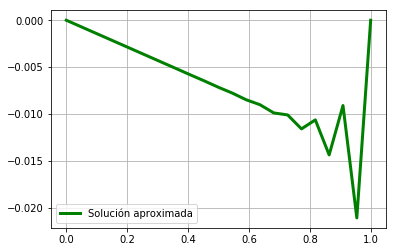
\includegraphics[width=0.47\linewidth]{conv-dif-centrado}&
    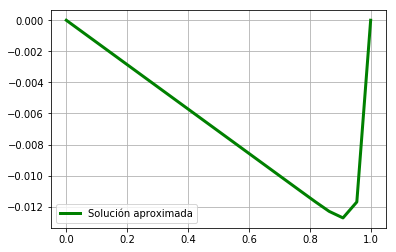
\includegraphics[width=0.47\linewidth]{conv-dif-descentrado}
    \\
    \small Diferencias finitas centradas
    &
    \small Diferencias finitas aguas arriba
  \end{tabular}
\end{center}
\item Modificar la función anterior para que
  \begin{itemize}
  \item Acepte tanto valores positivos como negativos para la
    convección, por ejemplo en el intervalo $[-200,200]$.
  \item Utilice un esquema descentrado aguas arriba cuando la convección
    es positiva y un esquema centrado aguas abajo cuando la convección
    sea negativa\footnote{Idea: definir distintos valores en la matriz
      tridiagonal, según los casos $c<0$ y $c\ge 0$.}
  \item ¿Qué resultados se obtienen? Muestra algún ejemplo con $c<0$.
  \end{itemize}
\end{itemize}

\subsubsection{Ejercicio 5}
Utilizando todo lo anterior, programar una función que resuelva
mediante el método de las diferencias finitas un problema de
convección-difusión en el \textbf{caso 2-dimensional}. Realizar test
numéricos similares a los descritos en los ejercicios 3 y 4.


\end{document}
%%% Local Variables:
%%% mode: latex
%%% TeX-master: t
%%% End:
